\chapter{Background}

\section{Software quality and duplicated code}

Software quality is hard to define. The term ``quality'' is ambiguous and is in the case
of software quality, multidimensional. Quality in itself has been defined as ``conformance
to requirements''~\cite[8]{crosby1980quality}. In software, a simple measure of
``conformance to requirements'' is correctness, and a lack of bugs. However, software
quality is often measured in other metrics, including metrics which are not directly
related to functionality~\cite[29]{MetricsAndModelsInSoftwareQuality}. Whenever duplicated
code needs to be changed, it might require changes in multiple locations, which leads to
metrics such as maintainability, analyzability and changeability being negatively
affected. Studies generally report that software projects contain $10-15\%$ duplicated
code, but some studies also report lower and higher percentages~\cite{CloningByAccident}.
Even so, the percentage of duplication is generally considered to be of non-trivial size
in many large code bases. Therefore, research into tools and techniques which can assist
in reducing duplicated code will be of benefit to almost all software.

Duplicated code can lead to a plethora of anti-patterns in software. Anti-patterns are bad
design decisions for software which can lead to technical debt. Technical debt occurs when
developers make technical compromises that are beneficial in the short term, but increases
complexity in the long-term~\cite[111]{TechnicalDebt}. An example of this, in the context
of duplicated code, is the ``Shotgun-Surgery'' anti-pattern~\cite[66]{fowlerrefactoring}.
This anti-pattern occurs when a developer wants to implement a change, but needs to change
code at multiple locations for the change to take effect. This is a typical situation
which slows down development and reduces maintainability when the amount of duplicated
code increases in a software project.

\section{Code clones}

Duplicated code is often described as ``code clones''. A pair of code snippets which are
duplicated are considered clones of each other.

\begin{definition}[Code snippet]
	A code snippet is a piece of contiguous source code in a larger software system.
\end{definition}

\begin{definition}[Code clone]
	A code clone is a code snippet which is equal to or similar to another code snippet. The two
	code snippets are both code clones, and together they form a clone pair.
	Similarity is determined by some metric such as number of equal lines of code.
\end{definition}

\begin{definition}[Clone class]
	A clone class is a set of code snippets where all snippets are considered clones of each
	other.
\end{definition}


The clone relation is a relation between code snippets which defines pairs of clones.
The clone relation is reflexive and symmetric, but not necessarily transitive. The transitive
property depends on the threshold for similarity when identifying code clones. Given

$$a \xleftrightarrow{clone} b \xleftrightarrow{clone} c$$


where $a,b,c$ are code snippets and $\xleftrightarrow{clone}$ gives the clone relation.
$a$ and $c$ are both clones of $b$, but not necessarily similar enough to be clones of
each other, depending on the threshold for similarity. If the threshold for similarity is
defined such that only equal clones are considered clones, the relation becomes
transitive, and clone classes are equal to the equivalence classes of the relation.

Code clones are generally classified into four types~\cite{Inoue_introduction_to_cc}. The
types would classify two code snippets as code clones with an increasing amount of
leniency. Therefore, type-1 code clones are very similar, while type-4 clones are not
necessarily syntactically similar at all. When defining types, it is the syntactic and
structural differences which is compared, not functionality. The set of code clones
classified by a code clone type is also a subset of the next type, meaning all type-1
clones are also type-2 clones, but not vice versa.

\textbf{Type-1} clones are syntactically identical. The only differences for a pair of
type-1 clones are elements without meaning, like comments and white-space, which is often
already ignored when source code is lexed and parsed. Figure \ref{fig:type1clone} shows an
example of a type-1 clone pair where only a comment and white-space is added to the
snippet on the right.

\begin{figure}[t]
	\begin{center}
        \begin{tabular}{p{5cm} | p{5cm}}
			\begin{lstlisting}
for (int i = 0; i < 10;   i++) {
    print(i);
}
\end{lstlisting} &
			\begin{lstlisting}
for (int i = 0; i < 10; i++) {
    // A comment

    print(i);
}
            \end{lstlisting}
		\end{tabular}
	\end{center}
    \caption{Type-1 clone pair}
    \label{fig:type1clone}
\end{figure}


\textbf{Type-2} clones are structurally identical. Possible differences include changes to
identifiers, literals and types. Type-2 clones are not much harder to detect than type-1
clones, since consistently renaming identifiers, literals and types allow a type-1
detection algorithm to find type-2 clones~\cite{Bakerdup}. This type of clone is relevant
to consider in refactoring scenarios when merging code clones as they can be relatively
simple to parameterize in order to merge two clones with for example differing literals.
The original locations of clones can then be replaced with a call to the merged code with
different parameters. Figure \ref{fig:type2clone} shows an example of a type-2 clone pair
where the numbers in the for loop initialization and condition could be parameterized to
correctly merge the two clones.

\begin{figure}[t]
	\begin{center}
        \begin{tabular}{p{5cm} | p{5cm}}
\begin{lstlisting}
for (int i = 0; i < 10; i++) {
    print(i);
}
\end{lstlisting} & \begin{lstlisting}
for (int (*\textbf j*) = (*\textbf 5*); (*\textbf j*) < (*\textbf 20*); (*\textbf j++*)) {
    print((*\textbf j*));
}
\end{lstlisting}
		\end{tabular}
	\end{center}
	\caption{Type-2 clone pair}
	\label{fig:type2clone}
\end{figure}

\textbf{Type-3} clones are required to be structurally similar, but not equal. Differences
include statements that are added, removed or modified. This clone type relies on a
threshold $\theta$ which determines how structurally different snippets can be in order to
be considered type-3 clones~\cite[6]{Inoue_introduction_to_cc}. The granularity for this
difference could for example be based on the number of differing tokens or lines.
Detecting this type of clone is generally computationally harder than detecting type-1 and
type-2 clones. Figure \ref{fig:type3clone} shows two code snippets where the code snippet
on the right has an added statement. In this example there is a one line difference
between the two snippets, so if the similarity is based on differing lines and $\theta
\geq 1$, the two snippets would be considered Type-3 clones.

\begin{figure}[t]
	\begin{center}
        \begin{tabular}{p{5cm} | p{5cm}}
			\begin{lstlisting}
for (int i = 0; i < 10; i++) {
    print(i);
}
\end{lstlisting} &
			\begin{lstlisting}
for (int i = 0; i < 10; i++) {
    print(i);
    (*\textbf{print(i*2);}*)
}
\end{lstlisting}
		\end{tabular}
	\end{center}
    \caption{Type-3 clone pair}
    \label{fig:type3clone}
\end{figure}



\textbf{Type-4} clones have no requirement for syntactical or structural similarity, but
are generally only relevant to detect when they have similar functionality. Detecting this
type of clone is very challenging, but attempts have been made using program dependency
graphs~\cite{SeedType4Detection}. Figure \ref{fig:type4clone} shows two code snippets
which have no clear syntactic or structural similarity, but is functionally equal.

\begin{figure}[t]
	\begin{center}
        \begin{tabular}{p{5cm} | p{5cm}}
			\begin{lstlisting}
print((n*(n-1))/2)
\end{lstlisting} &
			\begin{lstlisting}
int sum = 0;
for (int i = 0; i < n; i++) {
    for (int j = i+1; j < n; j++) {
        sum++;
    }
}
print(sum);
\end{lstlisting}
		\end{tabular}
	\end{center}
    \caption{Type-4 clone pair}
    \label{fig:type4clone}
\end{figure}


Type-1 clones are often referred to as ``exact'' clones, while Type-2 and Type-3 clones
are referred to as ``near-miss'' clones~\cite[1]{Zibran_real_time_search}.

\section{Code clone detection process and techniques}

\textbf{The Code clone detection process} is generally split into (but is not limited to)
a sequence of steps to identify clones~\cite{Inoue_introduction_to_cc}. This
process is often a pipeline of input-processing steps before finally comparing fragments
against each other and filtering. The steps are generally as follows:

\begin{enumerate}
	\item \textbf{Pre-processing}: Filter uninteresting code that we do not want to
	      check for clones, for example generated code. Then partition code into a set of
	      fragments, depending on granularity such as methods, files or lines.
	\item \textbf{Transformation}: Transform fragments into an intermediate
	      representation, with a source-map which gives the location to the original code.
          An algorithm could potentially do multiple transformation before arriving at the wanted
          representation
	      \begin{enumerate}
		      \item Extraction: Transform source code into the input for the comparison
		            algorithm. Can be tokens, AST, dependency graphs, suffix tree, etc.
		      \item Normalization: Optional step which removes superficial differences such as
		            comments, whitespace and identifier names. Often useful for detecting type-2
		            clones.
	      \end{enumerate}
	\item \textbf{Match detection}: Perform comparisons which outputs a set of
	      candidate clone pairs.
	\item \textbf{Source-mapping / Formatting}: Convert candidate clone pairs from the transformed
	      code back to clone pairs in the original source code.
	\item \textbf{Post-processing / Filtering}: Ranking and filtering manually or with
	      automated heuristics
	\item \textbf{Aggregation}: Optionally aggregating sets of clone pairs into clone sets
\end{enumerate}

\paragraph{Matching techniques} are the techniques used in the matching stage of the
algorithm which pairs fragments as clone-pairs. Most matching technique will also require
specific pre-processing to be done in the earlier steps, for example building an AST. Some
of the most explored techniques are as follows~\cite{ComparisonAndEvaluationOfTechniques}:

\paragraph{Text-based} approaches do little processing of the source code before
comparing. Simple techniques such as fingerprinting or incremental hashing have been used
in this approach. 

\paragraph{Token-based} approaches transform source code into a stream of tokens, similar
to lexical scanning in compilers. The token stream is then scanned for duplicated
subsequences of tokens. Since lexers often filter out superficial differences such as
whitespace, indentation and comments, this approach is more robust to such differences.
Concrete names of identifiers and values can be abstracted away when comparing the
token-stream, therefore type-2 clones can easily be identified. Type-3 clones can also be
identified by comparing the fragments tokens and keeping clone pairs with a lexical
difference lower than a given threshold. This can be solved with dynamic
programming~\cite{BakerSparseDynamicProgramming}. A common approach to detect clones using
token-streams is with a suffix-tree~\cite{Bakerdup}. A suffix-tree can solve the
\textit{Find all maximal repeats} problem efficiently, which essentially is the same
problem as finding clone pairs~\cite[143]{AlgorithmsOnStringsTreesSequences}. A suffix
array can also be used instead, which requires less
memory~\cite{ReplaceSuffixTreeWithEnchancedSuffixArray}. This type of code clone detection
is very fast compared to more intricate types of matching techniques.

\paragraph{Syntactic} approaches transform source code into either concrete syntax trees
or abstract syntax trees and find clones using either tree matching algorithms or
structural metrics. For tree matching, the common approach is to find similar subtrees,
which are then deemed as clone pairs. One way of finding similar subtrees is to compare
subtrees with a tolerant tree matching algorithm for detecting type-3
clones~\cite{ASTCloneDetection}. Variable names, literal values and types may be
abstracted to find type-2 clones more easily. Metrics-based techniques gather metrics for
code fragments in the tree and uses the metrics to determine if the fragments are clones
or not. One way is to use fingerprint functions where the fingerprint includes certain
metrics, and compare the fingerprints of all fragments to find clones~\cite{Deckard}.

\paragraph{Hybrid} approaches combine multiple approaches in order to improve detection
capabilities. For example a common approach which Zibran et
al.~\cite{Zibran_real_time_search} has implemented is a hybrid algorithm combining both
token-based suffix trees for type-1 and type-2 clone detection, with the dynamic
programming algorithm~\cite{BakerSparseDynamicProgramming} for type-3 clone detection.
Another example of a hybrid approach is the tool named
Siamese~\cite{SiameseScalableAndIncrementalClone}, which uses multiple intermediate
representations to get a better accuracy for clone detection.


\section{Incremental clone detection}

Incremental clone detection avoids computation of already computed results when performing
code clone detection on consecutive revisions of a code base.  A revision of a code base
is one version of a code base which has been changed from a previous revision, and once
edited, becomes the next revision.  A revision of the code base could for example be a
certain Git commit of the code base, or one could say a new revision of the code base is
created for each edit performed while programming. These two scenarios have respectively
been called the evolution scenario and the IDE
scenario~\cite{GodeIncrementalCloneDetection}. Incremental clone detection could be
realized in the form of either storing clones between each revision, or by maintaining a
data structure which is fast to update when the input updates, and also facilitates fast
extraction of clones. Since in most cases, an entire code base will not change drastically
in consecutive revisions, many code clones and the general structure of most of the source
code will remain, and therefore a lot of processing can be avoided. However, this is not a
simple problem, since changes in a single location can affect clone detection results
across the entire codebase.

In order to incrementally detect code clones, an initial algorithm computes the initial
clones, and for successive revisions of the source code, this list is incrementally
updated by an incremental algorithm. In some cases, this could be the same algorithm, but
in general the incremental algorithm is faster than the initial algorithm, and maintains
dynamic structures to perform efficient updates. 

Göde and Koschke proposed the first incremental clone detection
algorithm~\cite{GodeIncrementalCloneDetection}. The algorithm employs a generalized suffix
tree in which the amount of work of updating is only dependent on the size of the edited
code. This approach requires a substantial amount of memory, and is therefore limited in
scalability.

Nguyen et al.~\cite{LocalitySensitiveHashingIncremental} showed that an AST-based approach
utilizing ``Locality-Sensitive Hashing'' can detect clones incrementally with high
precision, and showed that incremental updates could be done in real-time ($< 1$ second)
for source code with a size of 300KLOC (lines of code).

Hummel et al.~\cite{IndexBasedIncrementalCloneDetection} later introduced the first
incremental and distributed clone detection technique for type-1 and type-2 clones. This
approach utilizes a custom ``clone index'' data structure which can be updated
efficiently. The implementation of this data structure is similar to that of an inverted
index. This technique uses distributed computing to speed up its detection process.

More recently, Ragkhitwetsagul and Krinke~\cite{SiameseScalableAndIncrementalClone}
presented the tool Siamese, which as mentioned uses a novel approach of having multiple
intermediate representations of source code to detect a high number of clones with support
for incremental detection. The tool can detect up to type-3 clones, but will only return
clones based on ``queries'' given to it by the user, and therefore does not allow listing
all clones in the code base. Queries are either files or methods in source-code, which are
then matched with other code clones.

\section{Code clone IDE tooling}

Developers are not always aware of the creation of clones in their code. \emph{Clone-aware
development} means including clone management as a part of the software development
process~\cite{Zibran_real_time_search}. Clone-aware development therefore requires
programmers to be aware of and be able to identify code clones while programming. Since
large software projects can contain a lot of duplication, it can be hard to keep track of
and manage clones. Tools which help developers locate and deal with clones can be a
solution to this. However, Rieger et al. claims that a problem with many detection
tools is that the tools ``report large amounts data that must be treated with little tool
support''~\cite[1]{InsightsSystemWideDuplication}. Detecting and eliminating clones early
in their lifecycle with IDE integrated tools could be a solution to the problem of dealing
with too many clones.

There are multiple existing clone detection tools which integrates into IDEs. The
IDE-based tools which exist can be categorized as
follows~\cite[8]{Udding_Towards_Convenient_Management}:

\begin{itemize}
	\item\textit{Copy-paste-clones:} This category of tools deals only with code snippets which are
	copy-pasted from another location in code. These tools therefore only track clones which
	are created when copy-pasting, and does not use any other detection techniques. Therefore,
	this type of tool is not suitable for detecting clones which are made accidentally, since
	developers are aware that they are creating clones when pasting already existing code
	snippets.

    \item\textit{Clone detection and visualization tools:} This category of tools has more
        sophisticated clone detection capabilities and will detect all code clones
        algorithmically, unlike copy-paste clone tools.

    \item\textit{Versatile clone management:} This category of tools covers tools which
        provide more services than the above. Services like refactoring and simultaneous
        editing of clones fall under this category.

\end{itemize}

The following tools have been developed as IDE tools to allow for clone-aware development:

\begin{itemize}

    \item Zibran et al. introduced a hybrid technique for performing real-time focused
        searches, i.e. searching for code clones of a selected code
        snippet~\cite{Zibran_real_time_search}. This technique can also detect Type-3
        clones. This algorithm was later implemented in the tool
        SimEclipse~\cite{Udding_Towards_Convenient_Management} which is a plugin for the
        Eclipse editor. This tool is also based on a suffix tree, but it is unclear if
        this suffix tree is updated incrementally.

    \item Another tool, SHINOBI, which is a plugin for the Visual Studio editor, can
        detect code clones in real-time without the need of the developer to select a code
        snippet~\cite{SHINOBI}. However, the clones being displayed seem to only be clones
        of the source-code which is currently being edited. This is limiting if a
        developer is searching for locations of clones, as they cannot simply look up the
        location of all clones. SHINOBI can detect type-1 and type-2 code clones and uses
        a token-based suffix array approach to detect clones. The paper does not describe
        how the suffix array is updated, but as the paper was released before the first
        paper describing dynamic suffix arrays~\cite{DynamicExtendedSuffixArrays}, one can
        assume that the suffix array is recomputed from scratch in each search.

    \item The modern IDE IntelliJ has a built-in duplication detection and refactoring
        service, it is able to detect type-1 and (some) type-2 code clones at a method
        granularity and can refactor to remove a clone-pair by replacing one of the clones
        with a method call to the other. The service does not seem to perform incremental
        updates.

\end{itemize}

\section{The Language Server Protocol}

Static analysis tools that integrate with IDEs are often tightly coupled to a specific IDE
and its APIs, like parsing and refactoring support. This makes it difficult to utilize a
tool in another IDE, since the APIs are no longer available. In order to make IDE-based
static analysis tools more widely available, it is therefore useful for such tools to be
made IDE agnostic. The Language Server Protocol (LSP) is a server-client protocol which
attempts to solve this problem~\cite{lsp}.

LSP is a protocol which specifies interaction between a client (IDE) and server (analysis
tool) in order to provide language tooling for the client. The goal of the protocol is to
avoid multiple implementations of the same language tools for every IDE and every
language, allowing for IDE agnostic tooling. Servers which implement LSP will be able to
offer IDEs code-completion, error-messages, go-to-definition and more. LSP also specifies
generic code-actions and commands, which the LSP server communicates to the client in
order to perform custom actions defined by the server.

Figure \ref{fig:lspcommunication} shows a sample interaction between client and server
using LSP. The client sends requests to a server in the form of JSON-RPC messages, and the
server sends a corresponding response, also in the form of JSON-RPC messages.

\begin{figure}[t]
	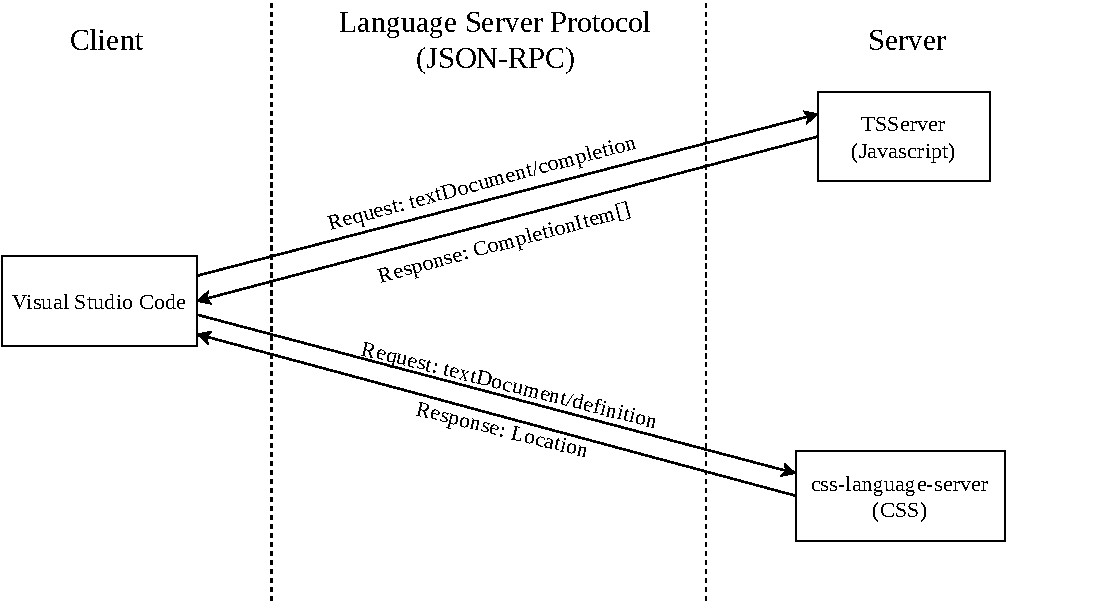
\includegraphics[width=\textwidth]{figures/lspcommunication.drawio.pdf}
	\caption{Example client-server interaction using LSP}
	\label{fig:lspcommunication}
\end{figure}

\section{Preliminary algorithms and data structures}
\label{prelimalgos}

Before our implementation is discussed, we will look at some preliminary algorithms and
data structures which may provide useful insights in the following chapters.

\subsection*{Parsing and incremental-parsing}

One of the first steps in most interpreters and compilers is to perform lexing and parsing
on the source code. Lexing is the process of turning the source code into a set of tokens,
turning strings such as ``if'', ``while'', ``+'' and ``('' into singular values which are
easier to work with. After the source code has been converted to a token-stream, the next
step is to parse the source code into a tree structure called a syntax tree. A syntax tree
is a tree which describes the structure of a program. For example an if-statement would
usually be a node in the tree, with a condition and a list of statements as children. An
abstract syntax tree (AST) is a tree where some details of the grammar may be left out in
the tree structure, such as having concrete nodes of tokens such as ``('' and ``)'', which
does not matter in a compiler or interpreters understanding of the program.

When parsing a program, the parser often relies on a grammar for the language, which
specifies the structure of the syntax tree, and is usually given in the form of a BNF
grammar. Given a BNF grammar, one could either write a parser which conforms to this
grammar (often recursive-descent for LL(1) grammars), or use a parser generator, which
generates the parser, given the grammar of the language. Parser generators can often
generate parser which are more complex, which allows for more complex grammars, such as
LALR(1) or LR(1) grammars.

A syntax tree is not only used for interpreting or compiling a language, it is also used
to perform static analysis on the program. Static analysis is an analysis performed
without running the program, and is often done in compilers in order to do for example
type-checking or data-flow analysis. Syntax trees are in essence very useful to traverse
or search a programs structure to look for certain properties of nodes or subtrees. 

In our detection algorithm we will need to be able to parse our source code into an AST
representation in order to select specific syntactic regions and extract the tokens.
Therefore, we need a parsing algorithm. For an incremental scenario, a useful observation
is that when a small edit is applied to a program, the syntax tree will usually not change
too much. When source code is edited it would therefore be more efficient to use an
incremental parsing algorithm which reuses parts of the old syntax tree, but updates it to
reflect the new source code. Incremental parsing is the process of parsing only parts of a
syntax tree whenever an edit is performed in a file, and reusing subtrees of the previous
syntax tree which did not change. The motivation behind incremental parsing is to have a
readily available syntax tree after every edit, while doing as little computing as
possible to maintain it.

Tree-sitter is a parser generator tool which specializes in incremental parsing. It
supports incremental parsing, error recovery and querying for specific nodes and
subtrees~\cite{treesitter}. These features combined makes Tree-sitter a powerful tool for
editing and has been used for IDE features such as syntax-highlighting, refactoring and
code navigation.

The incremental parsing algorithm in Tree-sitter\footnote{For a preliminary introduction
to Tree-sitter incremental parsing, see the following conference talk:\\
\url{https://www.thestrangeloop.com/2018/tree-sitter---a-new-parsing-system-for-programming-tools.html}}
is inspired by and implemented similarly to Wagner's incremental parsing
algorithm~\cite{PracticalAlgorithmsForIncremental}. Each node in the AST is decorated with
information on the range which it covers in the original source code. Whenever an edit is
performed at location $x$ in the source code, a new AST is built by first marking all the
nodes where the range of the node contains the position $x$. If a node contains the
position $x$ and is marked, it needs to be parsed again, but subtrees rooted in nodes
which are not marked can be reused, and can therefore be reused. Figure
\ref{fig:incrementalparsing} shows on the left an expression and its corresponding AST. If
the expression were to be changed to the expression on the right, the AST on the left
could be incrementally parsed by parsing only the marked nodes, and reusing all the other
nodes. Especially with the right-most difference node, we see how reusing an entire
subtree in the AST could save time compared to normal parsing. In larger programs we can
see significantly more reusage of subtrees, since an edit to a few lines would likely
require few nodes to be parsed compared to the number of nodes reused.

\begin{figure}[t]
    \begin{center}
        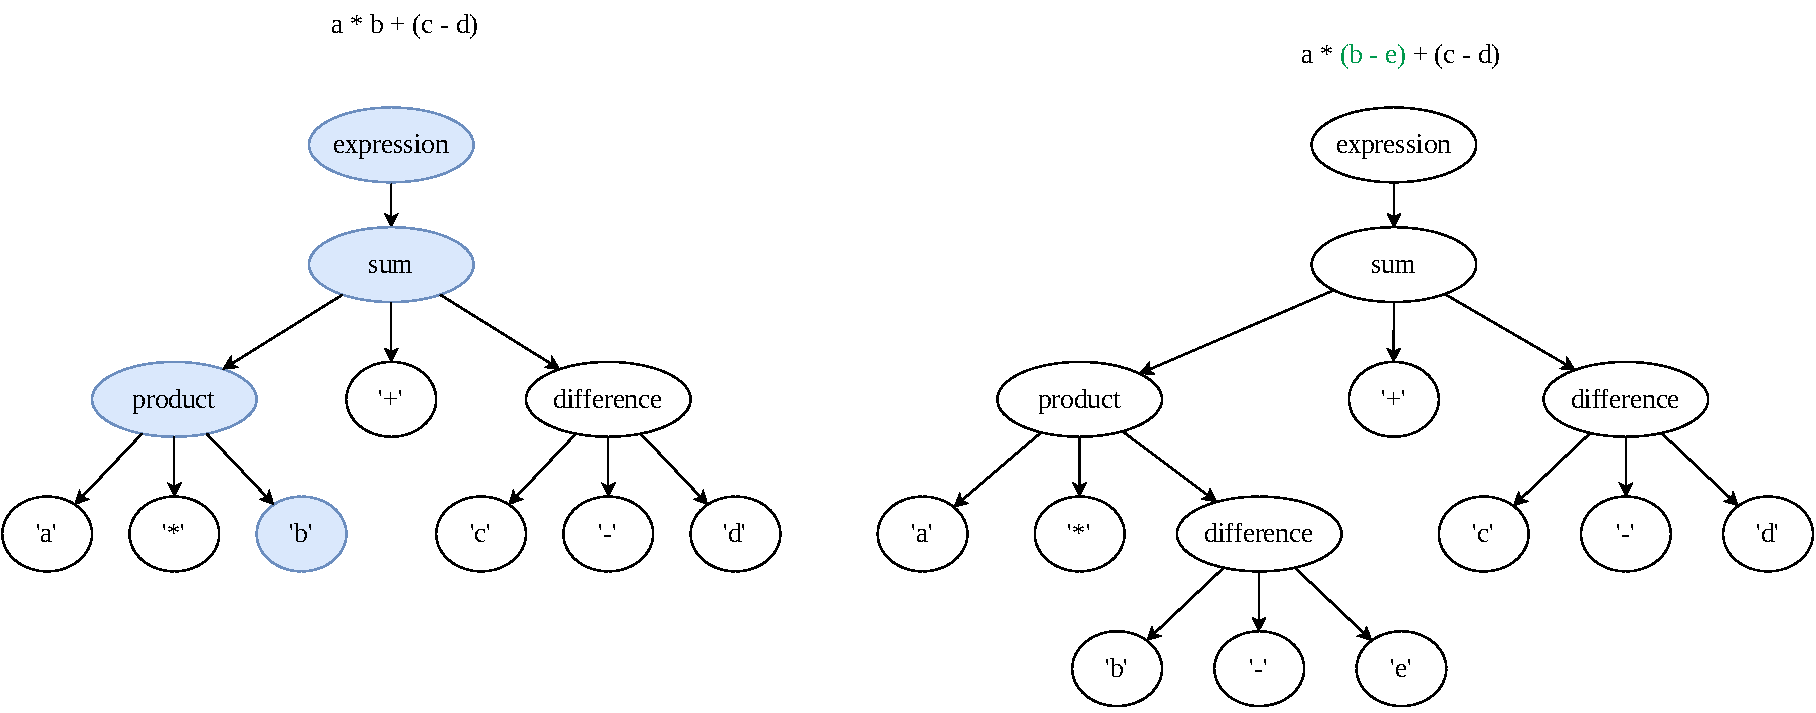
\includegraphics[width=1\textwidth]{figures/incrementalparsing.drawio.pdf}
    \end{center}
    \caption{AST's of two expressions. Left AST could be incrementally parsed to
        the right AST if marked nodes are parsed again and the rest of the tree is reused.}
    \label{fig:incrementalparsing}
\end{figure}


\subsection*{Suffix trees}

A classic algorithm for code clone detection traverses a suffix-tree in order to find
maximal repeats in all suffixes of the input string T~\cite{Zibran_real_time_search,
GodeIncrementalCloneDetection}. While our algorithm is only related to suffix trees, this
section gives some insight into the most common algorithm for clone detection.

The suffix tree of a string $T$ is a compressed trie where all the suffixes of $T$ have
been inserted into it. The trie is compressed by compressing consecutive nodes in a row
which have only one child into a single node. A common usage of a suffix tree is to
determine whether or not a suffix exists in $T$, and where in $T$ the suffix starts.

Figure \ref{fig:suffixtree} shows the suffix-tree for $T=\text{BANANA\$}$. In order to
determine where the suffix $\text{ANANA\$}$ exists in $T$, one can start from the root,
and traverse the tree, choosing the child node which correspond to the next character of
the suffix which has not been ``matched'' yet.

$$
\text{root} \xrightarrow{A} \text{node} \xrightarrow{\text{NA}} node \xrightarrow{\text{NA\$}} 1
$$

Following this path, we see that the suffix $\text{ANANA\$}$ exists in $T$ at index $1$.

Suffix trees can be constructed in linear time with Ukkonen's algorithm which builds a
larger and larger suffix tree by inserting characters one by one and utilizing some tricks
to avoid inserting suffixes before it needs to, lowering the complexity~\cite{Ukkonen}.

This data structure also facilitates solving the maximal repeat problem. A repeat in a
string T is a substring that occurs at least twice in T. A maximal repeat in T is a repeat
which is not a substring of another repeat in T, meaning that the maximal repeat cannot be
extended in any direction to form a bigger repeat. The problem of finding all maximal
repeats can be solved with a suffix tree using the following theorem:

\begin{theorem}[Repeats in suffix tree]

    Every internal node (except for the root) in a suffix tree corresponds to a substring
    which is repeated at least twice in T. The substring is found by concatenating the
    strings found on the path from the root of tree to the internal node.

\end{theorem}

This theorem is explained by the fact that any internal node has at least two children, and a
node having two children means that two suffixes share the same prefix up to that point.
An algorithm which finds the maximal repeats would find the internal nodes which
represents the longest strings. 

The classic algorithm~\cite{Zibran_real_time_search, GodeIncrementalCloneDetection} in
terms of finding duplication in a string (such as source code) using suffix trees would
find all repeats of length $k$, where $k$ is the threshold for how long a clone needs to
be. This can be found by traversing the suffix tree and looking at all internal nodes
which represent a string of length $\geq k$. Every internal node which represents a string
which is $\geq k$ would correspond to a substring of the source code which occurs at least
twice. Finding where the duplication occurs can be done by finding all the leaves of the
subtree rooted in the internal node, which each hold the position where the suffix starts in
T. Since a substring can have multiple repeats of different lengths longer than $k$,
different strategies can be used to select which substrings are selected or not, such as
filtering out repeats which are not maximal or repeats which contain or overlap each other.

In figure \ref{fig:suffixtree}, there are three repeats, ANA, A and NA. The only maximal
repeat would be ANA, since A and NA are not maximal.


\begin{figure}
	\begin{center}
		\begin{tikzpicture}[every tree node,
				level distance=1.25cm,sibling distance=1cm,
				edge from parent path={(\tikzparentnode) -- (\tikzchildnode)}]
			\Tree
			[.\addcircle{}
                \edge node[midway, above, sloped] {\$};
                [.\addsquare{6} ]
                \edge node[midway, below, sloped] {BANANA\$};
                [.\addsquare{0} ]
                \edge node[midway, above, sloped] {A};
                [.\addcircle{}
                    \edge node[midway, above, sloped] {\$};
                    [.\addsquare{5} ]
                    \edge node[midway, above, sloped] {NA};
                    [.\addcircle{}
                        \edge node[midway, above, sloped] {\$};
                        [.\addsquare{3} ]
                        \edge node[midway, above, sloped] {NA\$};
                        [.\addsquare{1} ]
                    ]
                ]
                \edge node[midway, above, sloped] {NA};
                [.\addcircle{}
                    \edge node[midway, above, sloped] {\$};
                    [.\addsquare{4} ]
                    \edge node[midway, above, sloped] {NA\$};
                    [.\addsquare{2} ]
			    ]
			]
		\end{tikzpicture}
		\caption{Suffix tree for $T=\text{BANANA\$}$}
        \label{fig:suffixtree}
	\end{center}
\end{figure}

\subsection*{Suffix arrays}

The suffix array (SA) of a string T contains a lexicographical sorting of all suffixes in
T. The suffix array does not contain the actual suffixes, but it contains integers
pointing to the index where the suffix starts in T. Conversely, the inverse suffix array
(ISA) contains integers describing which rank the suffix at a given position has. The rank
of a suffix is its lexicographical ordering in $T$. ISA is therefore the inverse array
of SA, such that if $\text{SA}[i] = n$, then $\text{ISA}[n] = i$.

\begin{definition}[Suffix array] 
    Let T be a text of length N.
    The suffix array \texttt{SA} of T is an array of length N where $\text{SA}[i] = n$ if the
    suffix at $T[n..N-1]$ is the ith lexicographically smallest suffix in T.
\end{definition}

\begin{definition}[Inverse suffix array] 
    Let T be a text of length N.
    The inverse suffix array ISA of T is an array of length N where $ISA[i] = n$ if the
    suffix at $T[i..N-1]$ is the nth smallest suffix in T lexicographically.
\end{definition}

The Longest-common prefix (LCP) array describes how many common characters there are in a
prefix between two suffixes which are next to each other in the suffix array. Since the
suffix array represents suffixes in a sorted order, the prefix length between adjacent
suffixes in SA will be the longest possible common prefix for each suffix. These are the
values in the LCP array.

\begin{definition}[LCP array]
    Let T be a text of length N and SA be the suffix array of T.
    The LCP array of T is an array of length N where $\text{LCP[i] = n}$ if the suffix
    $\text{T[SA[i]..N]}$ and $\text{T[SA[i-1]..N]}$ has a maximal common prefix of length
    $\text{n}$. $\text{LCP[0]}$ is undefined or {0}.
\end{definition}

For example, in table \ref{table:BANANA}, the LCP value at position 3 contains the number
of characters in the longest-common prefix of suffixes starting at position 1 (ANANA\$)
and position 3 (ANA\$). These suffixes have 3 common characters in their prefix, therefore
the LCP value at position 3 is 3.

\begin{table}
	\begin{center}
        \subfloat[Suffixes]{
		\begin{tabular}{c | l }
			Index & Suffix   \\
			\hline
			0     & BANANA\$ \\
			1     & ANANA\$  \\
			2     & NANA\$   \\
			3     & ANA\$    \\
			4     & NA\$     \\
			5     & A\$      \\
			6     & \$       \\
    \end{tabular}}
		\hspace{1cm}
        \subfloat[Sorted suffixes]{\begin{tabular}{c | l}
			Index & Suffix   \\
			\hline
			6     & \$       \\
			5     & A\$      \\
			3     & ANA\$    \\
			1     & ANANA\$  \\
			0     & BANANA\$ \\
			4     & NA\$     \\
			2     & NANA\$   \\
    \end{tabular}}
		\hspace{1cm}
        \subfloat[SA, ISA and LCP]{\begin{tabular}{c | c | c | c}
                Index & SA & ISA & LCP \\
				\hline
                0     & 6  & 4   & 0\\
                1     & 5  & 3   & 0\\
                2     & 3  & 6   & 1\\
                3     & 1  & 2   & 3\\
                4     & 0  & 5   & 0\\
                5     & 4  & 1   & 0\\
                6     & 2  & 0   & 2\\
        \end{tabular}}
        \caption{$T=\text{BANANA\$}$}
        \label{table:BANANA}
	\end{center}
\end{table}


Suffix arrays can be constructed in linear time in terms of the length of T. Many suffix
array construction algorithms (SACA) have been discovered in the last
decade~\cite{SuffixArrayConstruction}, many of which run in linear time. An algorithm
which has been shown to be very efficient in practice is Nong and Chan's algorithm based
on recursive suffix sorting of smaller constructed strings, which will be used in our
initial detection algorithm~\cite{LinearTimeSuffixArraySAIS}. 

The extended or enhanced suffix array is the suffix array and the additional LCP array,
which has been shown to be as powerful as a suffix tree, in terms of what can be computed
with it in the same time complexity~\cite{ReplaceSuffixTreeWithEnchancedSuffixArray}. An
advantage of using a suffix array over a suffix tree is that it uses a smaller amount of
memory, as suffix trees needs to store a lot of pointers. The extended suffix array is the
major data structure which will be used in our detection algorithm to find duplicate code,
as explained in the upcoming implementation chapters.

 \subsection*{Dynamic bitsets}

A bitset is an array of bits, each bit representing either the value true or false. A bit
with the value of 1 is usually referred to as a set bit, and a value of 0 is referred to
as an unset or cleared bit. Operations on bitsets normally include at least an operation
for setting the value at a position, and an operation for looking up the value at a
position. Bitsets are useful for many problems, especially as a ``succinct data
structure''. A succinct data structure is a data structure which attempts to use an amount
of memory close to the theoretic lower bound, while still allowing effective queries on
it. For example for a string of length $n$, we could store up to $O(n \log_{}\sigma)$ bits
before the bit vector exceeds the size of the string itself, where $\sigma$ is the size of
the string's alphabet.

The most well known queries to perform on bitsets is the rank/select queries.

\begin{definition}[Rank query on bitset]

    A rank query $rank_1(i)$ on a bitset B, computes the number of set bits up to, but not
    including position $i$. Conversely, $rank_0(B)$ returns the number of unset bits up to
    position $i$.

\end{definition}
\begin{definition}[Select query on bitset]
    
    A select query $select_1(i)$ on a bitset B, computes the position of the ith set bit
    in B. Conversely, $select_0(i)$ returns the position of the ith unset bit in B.

\end{definition}

Jacobson's rank can perform rank/select queries on static bitsets in $O(1)$ time by
pre-computing all answers in a space efficient table~\cite{JacobsonsRank}.

In some cases it is also useful to have a dynamic bitset, a bitset where
insertions/deletions are supported as well.

\begin{definition}[Dynamic bitset]

    A dynamic bitset is a bitset which in addition to other operations allow inserting and
    deleting bits.

    An insert operation $insert(i, v)$ on a bitset B inserts the value v at position i in
    B, pushing all values at position $\geq i$ one position up.

    A delete operation $delete(i)$ on a bitset B removes the value at position i in B, pushing all
    values at position $> i$ one position down.

\end{definition}

A simple implementation of a dynamic bitset could implement the whole bitset as a single
array of bytes $B$, which allows for accessing values in $O(1)$ time, but insertions and
deletions take $O(n)$ time, where $n$ is the number of bits in $B$.

Another implementation which speeds up the insertions/deletions represents the bitset as a
balanced tree containing multiple smaller bitsets. To represent a bitset of $n$ bits, we
can divide the bits into smaller bitsets, such that $O(\frac{n}{\log(n)})$ bitsets each
contains $O(log(n))$ bits. Since the bitsets are now of size $O(log(n))$, insertions and
deletions take only $O(log(n))$ time. The bitsets reside at the leaves of our balanced
tree, and internal nodes contain only two integers, storing the number of bits in the left
subtree ($N$), and the number of set bits in the left subtree ($S$). To access, insert or
delete on index $i$, the tree is traversed to find the correct bitset where the ith bit is
located, where the operation is done at that position. Finding the correct bitset and
position is done by utilizing $N$ and $S$ in each node which is traversed. All operations
now run in $O(\log(n))$ time, since traversing the tree to the correct bitset takes
$O(\log(\frac{n}{\log(n)}))$ and performing the operation takes $O(\log(n))$ time. Keeping
the tree balanced is done by splitting a leaf-node bitset to two nodes when the leaf-node
bitset has reached a certain size (such as $2 \times \log(n)$) and rebalancing the tree
after the split. Similarly, when considering deletions, two leaf-node bitsets can be
merged to their parent node when their combined number of bits has decreased to $\log(n)$.

Figure \ref{fig:DynamicBitset} shows how a dynamic bitset tree is structured, and
Algorithm \ref{alg:dynbitaccess} shows how to access a value in the tree. Traversing the
tree to calculate rank and select queries can be done similarly by summing set bits in
left-subtrees (rank) or selecting which subtree to descend based on the number of set bits
(select).

\begin{figure}[t]
	\begin{center}
		\begin{tikzpicture}[every tree node,
				level distance=2cm,sibling distance=2cm,
				edge from parent path={(\tikzparentnode) -- (\tikzchildnode)}]
			\Tree
            [.\node[left, circle, draw, align=left, label={[align=left] above: $N = 8$\\$S = 3$}]{};
                \edge node[midway, above, sloped] {};
                [.\node[left, circle, draw, align=left, label={[align=left] above left:$N = 4$\\$S = 2$}]{};
                    \edge node[midway, above, sloped] {};
                    [.\addsquare{0101} ]
                    \edge node[midway, above, sloped] {};
                    [.\addsquare{0001} ]
                ]
                \edge node[midway, above, sloped] {};
                [.\node[left, circle, draw, align=right, label={[align=right] above right:$N = 4$\\$S = 1$}]{};
                    \edge node[midway, above, sloped] {};
                    [.\addsquare{0100} ]
                    \edge node[midway, above, sloped] {};
                    [.\addsquare{0000} ]
                ]
            ]
		\end{tikzpicture}
		\caption{Dynamic bitset}
        \label{fig:DynamicBitset}
	\end{center}
\end{figure}

\begin{algorithm}[htp]
  \SetAlgoLined\DontPrintSemicolon
    \algo{\access{node, i}}{
        \If{{\isLeaf{node}}}{
            \Return $\ArrayAccess{\Access{\Var{node}}{\Var{bitset}}}{\Var{i}}$
        }

        \If{$\Access{\Var{node}}{\Var{N}} \leq \Var{i}$}{
            \Return \access{$\Access{\Var{node}}{\Var{left}}, \Var{i}$}
        }

        \Return \access{$\Access{\Var{node}}{\Var{right}}, \Var{i} - \Access{\Var{node}}{\Var{N}}$}
    }

  \vspace{0.5cm}
  \caption{Accessing a value in a dynamic bitset}
  \label{alg:dynbitaccess}
\end{algorithm}

\subsection*{Wavelet tree and wavelet matrix}

We can extend the notion of rank and select queries to strings as well. 

\begin{definition}[Rank query on string]

    A rank query $rank_c(i)$ on a string $S$ computes the number of occurrences of a
    character $c$ in $S$ up to, but not including position $i$.

\end{definition}
\begin{definition}[Select query on string]

    A select query $select_c(i)$ on a string $S$, computes the position of the ith
    occurrence of a character $c$ in $S$. 

\end{definition}

The classic data structure to efficiently compute $rank$ and $select$ queries on strings
is the \textbf{wavelet tree}~\cite{WaveletTree}. The data structure is a binary tree where every
node consists of a bitset, and each level of the tree consists of the bits of a single
position in each character of the string. Each bitset in the wavelet tree can for example
be implemented as a dynamic bitset to allow insertions/deletions on a wavelet tree.

\begin{figure}[t]
	\begin{center}
		\begin{tikzpicture}[every tree node,
				level distance=2cm,sibling distance=1.25cm,
				edge from parent path={(\tikzparentnode) -- (\tikzchildnode)}]
			\Tree
            [.\node[draw,
                align=center]{\tabbedCenterstack{a b b b e f c a g d d\\0 0 0 0 1 1 0 0 1 0 0}};
                \edge node[midway, above, sloped] {};
                [.\node[draw, align=center]{\tabbedCenterstack{a b b b c a d d\\0 0 0 0 1 0 1 1}};
                    \edge node[midway, above, sloped] {};
                    [.\node[draw, align=center]{\tabbedCenterstack{a b b b a\\0 1 1 1 0}};
                        \edge node[midway, above, sloped] {};
                        [.\addsquare{a} ]
                        \edge node[midway, above, sloped] {};
                        [.\addsquare{b} ]
                    ]
                    \edge node[midway, above, sloped] {};
                    [.\node[draw, align=center]{\tabbedCenterstack{c d d\\0 1 1}};
                        \edge node[midway, above, sloped] {};
                        [.\addsquare{c} ]
                        \edge node[midway, above, sloped] {};
                        [.\addsquare{d} ]
                    ]
                ]
                \edge node[midway, above, sloped] {};
                [.\node[draw, align=center]{\tabbedCenterstack{e f g\\0 0 1}};
                    \edge node[midway, above, sloped] {};
                    [.\node[draw, align=center]{\tabbedCenterstack{e f\\0 1}};
                        \edge node[midway, above, sloped] {};
                        [.\addsquare{e} ]
                        \edge node[midway, above, sloped] {};
                        [.\addsquare{f} ]
                    ]
                    \edge node[midway, above, sloped] {};
                    [.\node[draw, align=center]{\tabbedCenterstack{g\\0}};
                        \edge node[midway, above, sloped] {};
                        [.\addsquare{g} ]
                        \edge node[midway, above, sloped] {};
                        [.\addsquare{h} ]
                    ]
                ]
            ]
		\end{tikzpicture}
		\caption{Wavelet tree for S = abbbefcagdd}
        \label{fig:wavelettree}
	\end{center}
\end{figure}


\begin{table}[t!]
	\begin{center}
		\begin{tabular}{c}
            \begin{tabular}{c c c c c c c c c c c c}
                a & b & b & b & e & f & c & a & g & d & d \\
                \hline
            \end{tabular} \\
            \begin{tabular}{c c c c c c c c c c c c}
                0 & 0 & 0 & 0 & 1 & 1 & 0 & 0 & 1 & 0 & 0
            \end{tabular} \\
            \begin{tabular}{c c c c c c c c|c c c}
                0 & 0 & 0 & 0 & 1 & 0 & 1 & 1 & 0 & 0 & 1
            \end{tabular} \\
            \begin{tabular}{c c c c c|c c c|c c|c}
                0 & 1 & 1 & 1 & 0 & 0 & 1 & 1 & 0 & 1 & 0
            \end{tabular} \\
		\end{tabular}
		\caption{Levelwise wavelet tree}
		\label{table:levelwisewavelettree}
	\end{center}
\end{table}




Figure \ref{fig:wavelettree} shows the wavelet tree for the string \verb|abbbefcagdd|. The
wavelet tree can perform $access$, $rank$ and $select$ queries by traversing the tree from
root to leaf. 

$access(i)$ gives the bitstring of the character at a position $i$ by first accessing
position $i$ in the root bitset, if the bit is a $0$, we traverse to the left, if it is a
$1$ we traverse to the right. Before traversing to a child, we compute $rank_0(i)$ or
$rank_1(i)$, depending on what bit is at position $i$, the resulting rank is the next
position to consider in the subtree. This is done recursively until a leaf-node is found,
and the bits which were examined at each node is the bitstring of the character at
position $i$.

$rank_c(i)$ traverses the tree similarly to $access(i)$, but we use the bits of $c$ to
guide us to the correct subtree. When a leaf-node is reached, the value of $i$ is
returned, since when a leaf is reached, $i$ will be pointing to the correct rank in the
fictitious bitset of only $c$ characters

The wavelet tree can be traversed in $O(\log \sigma)$ time where $\sigma$ is the size of
the alphabet. However, the $access$, $rank$ and $select$ operations also depend on how
fast the bitsets can perform $access$, $rank$ and $select$ operations. If the bitsets are
implemented using for example Jacobson's rank~\cite{JacobsonsRank}, the bitsets have a
$O(1)$ $access$, $rank$ and $select$ time, but if we require dynamic bitsets for
insertion/deletions, the time complexity increases to $O(\log n \log \sigma)$ because a
bitset operation which takes $O(\log n)$ time is required in each level of the tree.

The wavelet tree can also be implemented without pointers, known as a levelwise or
pointerless wavelet tree~\cite{LevelwiseWaveletTree}. Table \ref{table:levelwisewavelettree}
shows the levelwise wavelet tree, which can be traversed level by level, but determining
which interval of the bitset the node you are in occupies requires two calls to $rank$.
The details of the levelwise wavelet trees are out of scope for this thesis, but leads us
into the next wavelet data structure.

The \textbf{wavelet matrix} is a relatively recent improvement on the wavelet tree, which
has been shown to be more efficient for $access$, $rank$ and $select$ queries, as well as
less memory intensive for larger alphabets~\cite{WaveletMatrix}. As the name suggests, the
wavelet matrix is a matrix of bitsets, instead of a tree of bitsets. Similarly to the
levelwise wavelet tree, for a string $S$ of size $n$, each level of the matrix consists of
a bitset of size $n$. The difference between a levelwise wavelet tree and a wavelet matrix
is that the assumption that the "children" of an interval $[x, y]$ needs to occupy exactly
$[x, y]$ is no longer true. We can instead put all $0$ bits to the left in the next level,
and all $1$ bits to the right. For each level we store an integer $z_l$, which holds the
number of zero bits in level $l$. 

For $access$ operations, we traverse each level similarly to a levelwise wavelet tree, but
instead of traversing a smaller and smaller interval in each level, we simply look at the
current bit at position $i$, if it is a zero, the bit to examine in the next level is
$rank_0(i)$, if the bit is a $1$, the bit to examine in the next level is $z_l +
rank_1(i)$. $rank_c(i)$ operation is carried out similarly, but we also keep track of a
preceding position to the final $i$, which we subtract from $i$, to count only the number
of proceeding number of $a$ characters. Table \ref{table:waveletmatrix} shows an example
wavelet matrix, and algorithm \ref{alg:waveletmatrixaccess} and
\ref{alg:waveletmatrixrank} shows how $access$ and $rank$ operations can be carried out
for a wavelet matrix. The time complexities for $access$, $rank$ and $select$ operations
is the same as for wavelet trees.

\begin{table}[t]
	\begin{center}
		\begin{tabular}{c}
            \begin{tabular}{c c c c c c c c c c c c}
                a & b & b & b & e & f & c & a & g & d & d \\
                \hline
                0 & 0 & 0 & 0 & 1 & 1 & 0 & 0 & 1 & 0 & 0 \\
                0 & 0 & 0 & 0 & 1 & 0 & 1 & 1 & 0 & 0 & 1 \\
                0 & 1 & 1 & 1 & 0 & 0 & 1 & 0 & 1 & 1 & 0
            \end{tabular} \\
		\end{tabular}
		\caption{Wavelet matrix for S = abbbefcagdd}
		\label{table:waveletmatrix}
	\end{center}
\end{table}


\begin{figure}
\begin{minipage}{0.49\textwidth}
    \begin{algorithm}[H]
        \SetAlgoLined\DontPrintSemicolon
        \algo{\access{WM, i}}{
            $\Var{bits} \gets \textrm{empty\ list}$ \;
            $\Var{l} \gets 0$ \;
            \While{$\Var{l} < \Len{$\Var{WM}$}$}{
                \Add{$\Var{bits}, \access{$\ArrayAccess{\Var{WM}}{\Var{l}}, \Var{i}$}$} \;
                \uIf{$\access{$\ArrayAccess{\Var{WM}}{\Var{l}}, \Var{i}$} = 1$}{
                    $\Var{i} \gets z_l + \RankOne{$\ArrayAccess{\Var{WM}}{\Var{l}}, \Var{i}$}$ \;
                }
                \Else{
                    $\Var{i} \gets \RankZero{$\ArrayAccess{\Var{WM}}{\Var{l}}, \Var{i}$}$ \;
                }
                $\Var{l} \gets \Var{l} + 1$
            }
            \Return $\Var{bits}$ \;\;
        }

        \caption{Wavelet matrix access}
        \label{alg:waveletmatrixaccess}
    \end{algorithm}
\end{minipage}
\begin{minipage}{0.49\textwidth}
    \begin{algorithm}[H]
        \SetAlgoLined\DontPrintSemicolon
        \algo{\RankC{WM, i}}{
            $\Var{l} \gets 0$ \;
            $\Var{p} \gets 0$ \;
            \While{$\Var{l} < \Len{$\Var{WM}$}$}{
                \uIf{$\access{$\ArrayAccess{\Var{WM}}{\Var{l}}, \Var{i}$} = 1$}{
                    $\Var{i} \gets z_l + \RankOne{$\ArrayAccess{\Var{WM}}{\Var{l}}, \Var{i}$}$ \;
                    $\Var{p} \gets z_l + \RankOne{$\ArrayAccess{\Var{WM}}{\Var{l}}, \Var{p}$}$ \;
                }
                \Else{
                    $\Var{i} \gets \RankZero{$\ArrayAccess{\Var{WM}}{\Var{l}}, \Var{i}$}$ \;
                    $\Var{p} \gets \RankZero{$\ArrayAccess{\Var{WM}}{\Var{l}}, \Var{p}$}$ \;
                }
                $\Var{l} \gets \Var{l} + 1$
            }
            \Return $\Var{i} - \Var{p}$ \;
        }
        \caption{Wavelet matrix rank}
        \label{alg:waveletmatrixrank}
    \end{algorithm}
\end{minipage}
\end{figure}

The wavelet matrix is constructed level by level. In level $i$, the bit at position $i$ in
each character is inserted. Before constructing the next level, each character is sorted
by the current bit, so that all the characters with $0$ bits at position $i$ occupies the
left side of level $i + 1$, and vice versa for $1$ bits.

\subsection*{Burrows-Wheeler transform}

\begin{table}[t]
	\begin{center}
        \subfloat[Cyclic shifts]{
		\begin{tabular}{c | l }
			Index & Cyclic-shift   \\
			\hline
			0     & BANANA\$ \\
			1     & ANANA\$B \\
			2     & NANA\$BA \\
			3     & ANA\$BAN \\
			4     & NA\$BANA \\
			5     & A\$BANAN \\
			6     & \$BANANA \\
    \end{tabular}}
		\hspace{0.5cm}
        \subfloat[Sorted cyclic shifts and BWT]{\begin{tabular}{c | l}
			Index & Cyclic-shift   \\
			\hline
            6     & \$BANAN\textbf{A} \\
            5     & A\$BANA\textbf{N} \\
			3     & ANA\$BA\textbf{N} \\
			1     & ANANA\$\textbf{B} \\
			0     & BANANA\textbf{\$} \\
			4     & NA\$BAN\textbf{A} \\
			2     & NANA\$B\textbf{A} \\
    \end{tabular}}
		\hspace{0.5cm}
        \subfloat[LF function]{\begin{tabular}{c | l}
			L & F   \\
			\hline
            0     & $Rank_A(0) + C[A] = 0 + 1 = 1$\\
            1     & $Rank_N(1) + C[N] = 0 + 5 = 5$ \\
			2     & $Rank_N(2) + C[N] = 1 + 5 = 6$ \\
			3     & $Rank_B(3) + C[B] = 0 + 4 = 4$ \\
            4     & $Rank_{\$}(4) + C[\$] = 0 + 0 = 0$ \\
			5     & $Rank_A(5) + C[A] = 1 + 1 = 2$ \\
			6     & $Rank_A(6) + C[A] = 2 + 1 = 3$ \\
    \end{tabular}}
    \caption{S = BANANA\$, BWT = ANNB\$AA}
    \label{table:bwt}
	\end{center}
\end{table}

The Burrows-Wheeler transform (BWT) is a transform on strings, often performed to improve
compression and searching~\cite{BWT}. The transform is computed by sorting all
``cyclic-shifts'' of the string lexicographically and extracting a new string from the
last column of the cyclic-shift'' matrix. \$ is added to the string as a unique
terminating character, this makes some of the algorithms on the BWT simpler. \$ is always
the smallest character lexicographically. Table \ref{table:bwt} shows the BWT for the
string S = BANANA\$. There is a very tight correlation between the BWT of a string and its
suffix array, which is why this transform will be relevant for our detection algorithm.

\begin{definition}{Cyclic-shift}

    The cyclic-shift of order $i$ for a string $S$ is the cyclic-shift of $S$ such that
    all characters in $S$ are rotated $i$ characters to the left. The cyclic-shift of
    order $i$ is denoted $CS_i$

\end{definition}

\begin{definition}{Burrows-Wheeler transform}

    The Burrows-Wheeler transform of a string $S$ is a transformation on $S$ where the
    cyclic-shifts of $S$ are sorted, and the final character in each shift is concatenated.

\end{definition}

As mentioned, there is a tight correlation between the suffix array of S and the BWT of S.
Table \ref{table:bwt} also shows that the indices of the sorted cyclic-shifts correspond
to exactly the SA of S. This coincides because when sorting cyclic-shifts, everything that
occurs after the \$ of the cyclic-shift will not affect its lexicographical ordering. This
is because no cyclic-shift will have a \$ in the same position, so comparing two cyclic
shifts lexicographically will always terminate whenever a \$ is found. This means that the
ordering of cyclic shifts is essentially the same as sorting all suffixes of S. Algorithm
\ref{alg:bwt} shows how the BWT of S can be calculated directly from the SA of S in linear
time. Since this is a one to one correlation between the SA and BWT, dynamic updates to a
BWT would correspond to similar dynamic updates in the SA (and ISA). This will be useful
in the upcoming implementation chapters for the incremental code clone detection
algorithm.

\begin{algorithm}[htp]
  \SetAlgoLined\DontPrintSemicolon
    \algo{\ComputeBWT{S, SA}}{
        $\Var{n} \gets \Access{S}{len}$

        $BWT \gets \mathrm{string\ of\ length\ } n$

        \For{$i \From 0 \To \Var{n}$}{

            $\Var{pos} \gets (\SA{\Var{i}} - 1)\ \%\ n$

            $\BWT{i} = \ArrayAccess{\Var{S}}{pos}$
        }

        \Return BWT
    }

  \vspace{0.5cm}
  \caption{Calculating the BWT of a string T from its suffix array}
  \label{alg:bwt}
\end{algorithm}


An essential property of the BWT is that the transformation is reversible. By examining
the BWT of a string T, we see that the BWT is a permutation of S. We will also see that
there is a correlation between the characters in the first column of the cyclic-shift
matrix and the last column, which allows us to compute the original string, given only the
BWT.

$S$ can be computed from the BWT as long as there is a unique terminating character (\$),
or the position of the final character is stored. S is computed backwards by starting at
the final character ($S[n - 1]$) and then finding the cyclic-shift where that character
occurs in the first column (the previous cyclic-shift). The character in the last column
of that cyclic-shift is $S[n - 2]$. If there are multiple of the same character, the nth
occurrence of a certain symbol in the last column will map to the nth occurrence of the
same symbol in the first column. This process is repeated until we finish the cycle,
returning to the final character in the last column. Essentially, this process consists of
traversing cyclic-shifts backwards and looking at the final character, which will give us
S, since the final character of the cyclic-shift is continually shifting one position.

We can use the fact that the first column consists of the letters of S in sorted order to
determine the previous cyclic-shift with only the last column. We can calculate the
previous cyclic-shift from only the last column by determining how many characters are
lexicographically smaller than the current character, and also the rank of the current
character at this position. The sum of these two values is the location of the previous
cyclic-shift. This function is called the Last-to-first function (LF function).
Calculating the LF function can be done efficiently by using a rank/select data structure
such as a wavelet tree~\cite{WaveletTree} or wavelet matrix~\cite{WaveletMatrix} to
calculate the rank of all the characters in the BWT, and an array $C$ which contains the
number of occurrences of each letter in the BWT. In table \ref{table:bwt}, we can compute
the original $S$ from the BWT by starting at position $4$, because that is the position of
the \$, then use the LF-function, $LF(4) = 0$, which means the second to last character is
$BWT[0] = A$. $LF(0) = 1$, which means the next character is $BWT[1] = N$, and so on.

The LF function will also be useful in the detection algorithm where we dynamically update
the suffix array of $S$, given the changes of the BWT of $S$.
